\section{Appendix}

\subsection{Ethical Considerations}\label{appendix:ethical-considerations}
This study employs the Curlie dataset, managed by dedicated volunteers and moderators ensuring its content remains legal and free from marketing schemes. 
To further support these efforts, we are releasing the re-labeled datasets \texttt{curlie-gpt3.5-10k} and \texttt{curlie-gpt4-10k} to the public.

Additionally, we employed the \texttt{crowdsourced} dataset, originally created by Amazon Mechanical Turk workers for the homepage2vec paper \cite{homepage2vec}. 
These workers were compensated in accordance with ethical standards and minimum wage requirements set by the Fair Work platform \cite{ethics2}.


The use of LLMs for annotation, while efficient, raises concerns regarding the economic impact on human annotators who depend on such tasks for their livelihood. 
It is imperative to ensure that this process supplements, rather than replaces, human annotators. In this context, providing platforms like Dynamo \cite{ethics1} for Amazon Mechanical Turk workers to communicate and organize is crucial.
Additionally, it is crirical to maintain these principles and be cautious of influences from large entities that may hinder the efforts of workers to organize and advocate for their rights.

Moreover, the extensive datasets training LLMs may contain biases, potentially influencing the labeling process and perpetuating stereotypes or inequalities. 
It's essential to address these biases to maintain fairness and uphold ethical standards in automated systems.

\subsection{Crowdsourced Label Distribution}

\begin{figure}[!ht]
    \centering
    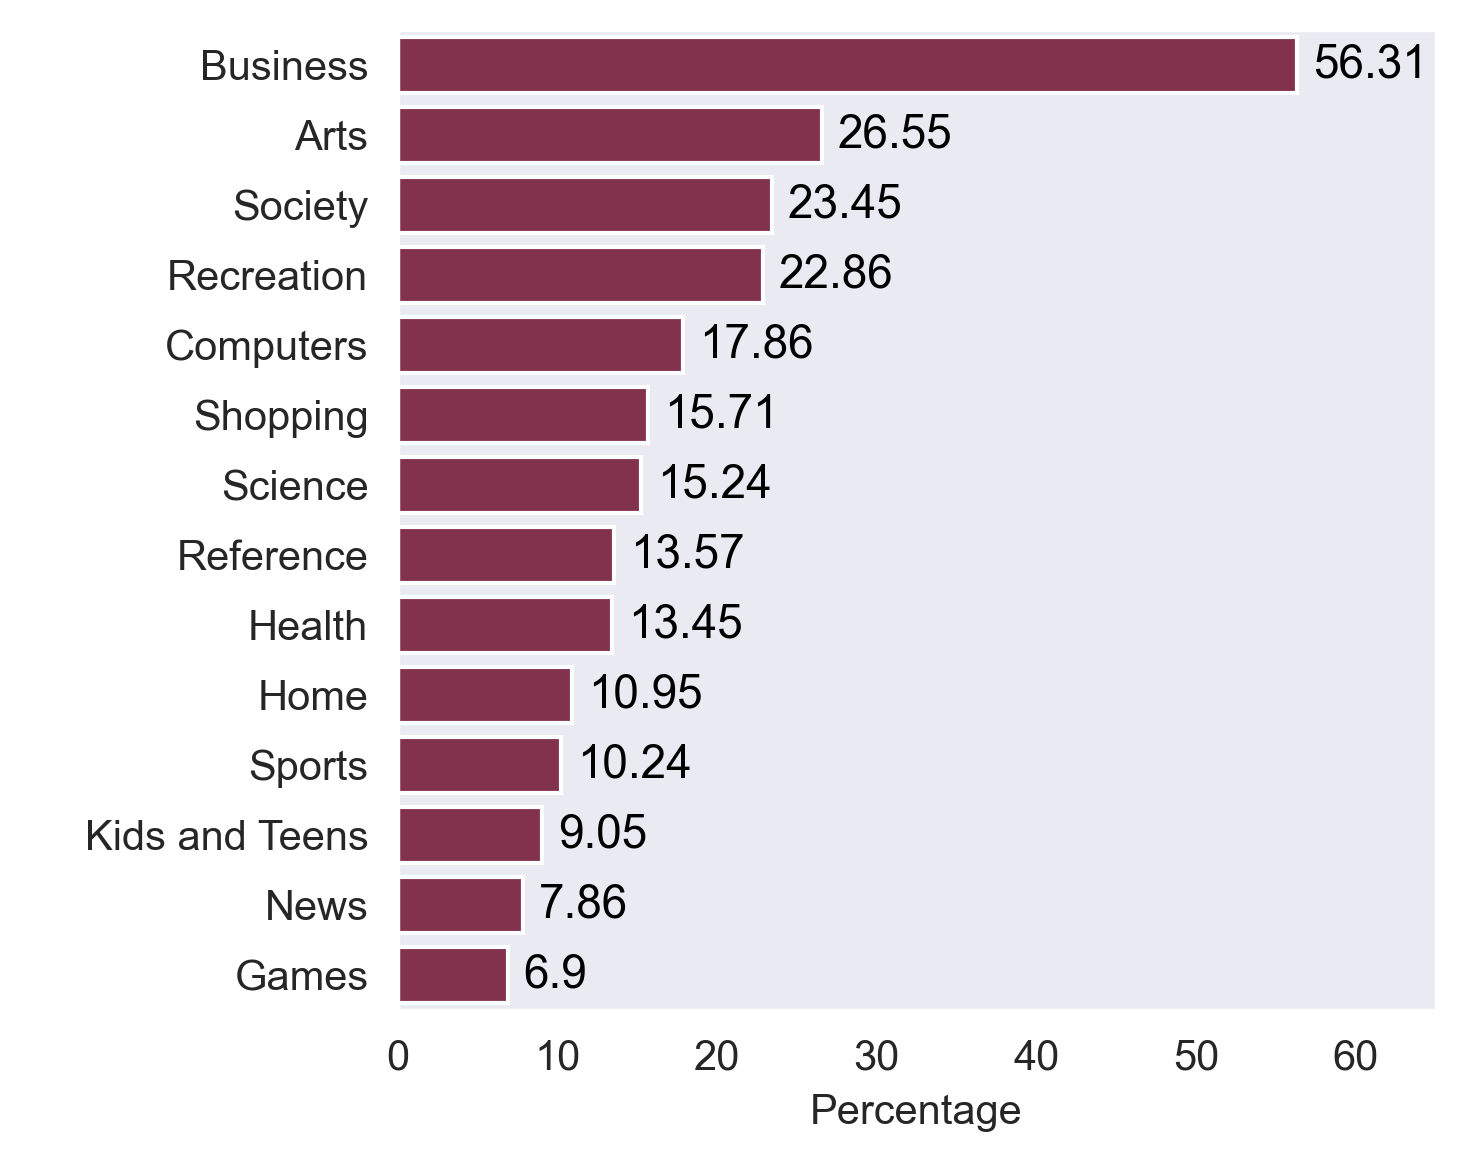
\includegraphics[width=0.4\textwidth]{./figures/category_distribution.png}
    \caption{Label distribution of the crowdsourced dataset.}
    \label{fig:label-distribution}
\end{figure}

\subsection{System prompt}\label{app:prompt}
This appendix details the GPT prompt used for website topic classification. 

\textbf{System Prompt:} 

\begin{lstlisting}
You are an expert in website topic classification that accurately predicts the topic. Analyze the provided website data and classify it into relevant categories.

[
    "Arts",
    "Business",
    "Computers",
    "Games",
    "Health",
    "Home", 
    "Kids_and_Teens",
    "News",
    "Recreation",
    "Reference",
    "Science", 
    "Shopping",
    "Society",
    "Sports"
]

Output a JSON string with categories as keys
and binary values (0 or 1) indicating if the 
webpage belongs to the topic. 

Always include all categories in the JSON
output.
\end{lstlisting}
\textbf{Example for a \texttt{1-shot} model:}
\begin{lstlisting}
Given website data:
{         
    "title": "The New York Times ...",
    "description": "Find breaking news ...",
    "keywords": [
        "breaking news", "...",],
    "links": ["breaking-news", "...",],
    "tld": "com",
    "domain": "nytimes.com",
    "metatags": ["NYT", "..."],
    "sentences": ["Breaking news: A major political development reshapes the landscape in Washington.", "...",]
}
    A good classification is:
{
    "Arts": 1,
    "Business": 1,
    "Computers": 0,
    "Games": 0,
    "Health": 1,
    "Home": 0,
    "Kids_and_Teens": 0,
    "News": 1,
    "Recreation": 0,
    "Reference": 0,
    "Science": 1,
    "Shopping": 0,
    "Society": 1,
    "Sports": 1
}
\end{lstlisting}


